\documentclass[journal]{IEEEtran}
\usepackage[a5paper, margin=10mm, onecolumn]{geometry}
\usepackage{lmodern} % Ensure lmodern is loaded for pdflatex
\usepackage{tfrupee} % Include tfrupee package

\setlength{\headheight}{1cm} % Set the height of the header box
\setlength{\headsep}{0mm}     % Set the distance between the header box and the top of the text

\usepackage{gvv-book}
\usepackage{gvv}
\usepackage{cite}
\usepackage{amsmath,amssymb,amsfonts,amsthm}
\usepackage{algorithmic}
\usepackage{graphicx}
\usepackage{textcomp}
\usepackage{xcolor}
\usepackage{txfonts}
\usepackage{listings}
\usepackage{enumitem}
\usepackage{mathtools}
\usepackage{gensymb}
\usepackage{comment}
\usepackage[breaklinks=true]{hyperref}
\usepackage{tkz-euclide} 
\usepackage{listings}                                      
\def\inputGnumericTable{}                                 
\usepackage[latin1]{inputenc}                                
\usepackage{color}                                            
\usepackage{array}                                            
\usepackage{longtable}
\usepackage{multicol}
\usepackage{calc}                                             
\usepackage{multirow}                                          
\usepackage{hhline}                                           
\usepackage{ifthen}                                           
\usepackage{lscape}
\begin{document}
	
\bibliographystyle{IEEEtran}
\vspace{3cm}
	
\title{10.4.ex.9}
\author{EE24BTECH11008 - Aslin Garvasis}
% \maketitle
% \newpage
% \bigskip
{\let\newpage\relax\maketitle}
	
\renewcommand{\thefigure}{\theenumi}
\renewcommand{\thetable}{\theenumi}
\setlength{\intextsep}{10pt} % Space between text and floats
	

\numberwithin{equation}{enumi}
\numberwithin{figure}{enumi}
\renewcommand{\thetable}{\theenumi}
	
	
\textbf{Question}:\newline
Find the roots of \( 4x^2 + 3x + 5 = 0 \) by the method of completing the square. \\
	

		\begin{figure}[h!]
		\centering
		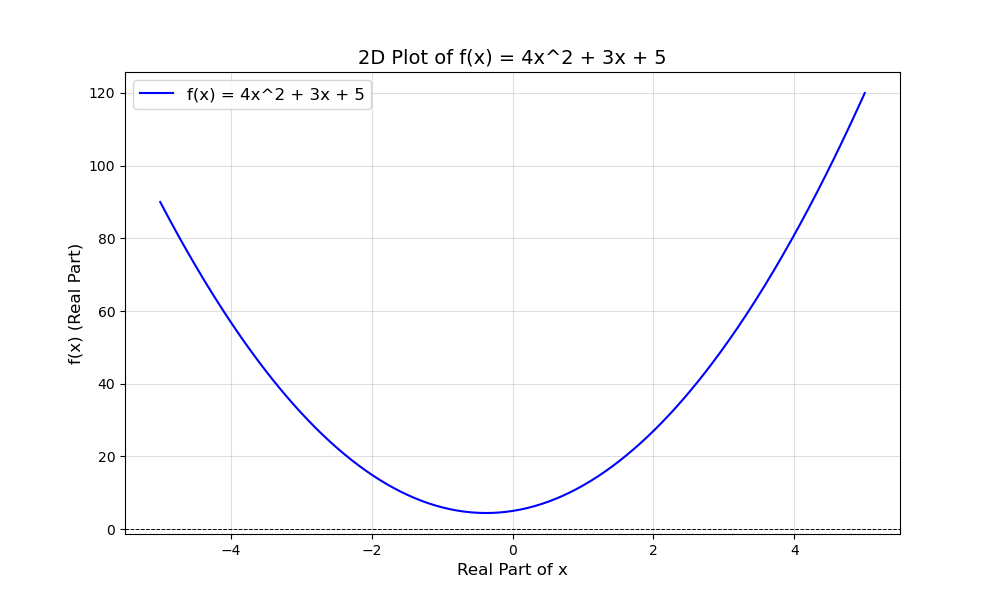
\includegraphics[width=\columnwidth]{figs/Fig1.png}
			\caption{Graphical representation of the function}
		\label{stemplot}
	\end{figure}
\section*{Solution (Completing the Square Method)}

The given quadratic equation is:

\begin{align}
4x^2 + 3x + 5 = 0
\end{align}

Step 1: Divide the equation by 4 to make the coefficient of \( x^2 \) equal to 1:

\begin{align}
x^2 + \frac{3}{4}x + \frac{5}{4} = 0
\end{align}

Step 2: Isolate the constant term:

\begin{align}
x^2 + \frac{3}{4}x = -\frac{5}{4}
\end{align}

Step 3: Complete the square. Take half the coefficient of \( x \), square it, and add it to both sides. The coefficient of \( x \) is \( \frac{3}{4} \), so:

\begin{align}
\left(\frac{3}{4} \cdot \frac{1}{2}\right)^2 = \left(\frac{3}{8}\right)^2 = \frac{9}{64}
\end{align}

Add \( \frac{9}{64} \) to both sides:

\begin{align}
x^2 + \frac{3}{4}x + \frac{9}{64} = -\frac{5}{4} + \frac{9}{64}
\end{align}

Step 4: Simplify both sides. The left-hand side becomes a perfect square trinomial:

\begin{align}
\left(x + \frac{3}{8}\right)^2 = -\frac{80}{64} + \frac{9}{64}
\end{align}

\begin{align}
\left(x + \frac{3}{8}\right)^2 = -\frac{71}{64}
\end{align}

Step 5: Solve for \( x \). Take the square root of both sides:

\begin{align}
x + \frac{3}{8} = \pm \sqrt{-\frac{71}{64}}
\end{align}

Since \( \sqrt{-1} = i \), we rewrite the equation as:

\begin{align}
x + \frac{3}{8} = \pm i \sqrt{\frac{71}{64}}
\end{align}

Simplify further:

\begin{align}
x + \frac{3}{8} = \pm i \frac{\sqrt{71}}{8}
\end{align}

Step 6: Solve for \( x \):

\begin{align}
x = -\frac{3}{8} \pm i \frac{\sqrt{71}}{8}
\end{align}

Step 7: Combine terms:

\begin{align}
x = \frac{-3 \pm i\sqrt{71}}{8}
\end{align}

Thus, the roots of the equation are:

\begin{align}
\boxed{x = \frac{-3 + i\sqrt{71}}{8}, \quad x = \frac{-3 - i\sqrt{71}}{8}}
\end{align}

\section*{Solution (Newton's Method)}

Newton's method is an iterative technique for finding approximations to the roots of a real-valued function. The iterative formula for Newton's method is given by:

\begin{align}
x_{n+1} = x_n - \frac{f(x_n)}{f'(x_n)}
\end{align}

where \( f(x) \) is the function for which we are solving \( f(x) = 0 \), and \( f'(x) \) is its derivative.

For the given quadratic equation \( 4x^2 + 3x + 5 = 0 \), let:

\begin{align}
f(x) = 4x^2 + 3x + 5
\end{align}

Then, the derivative is:

\begin{align}
f'(x) = 8x + 3
\end{align}

Substitute these into the Newton's method formula:

\begin{align}
x_{n+1} = x_n - \frac{4x_n^2 + 3x_n + 5}{8x_n + 3}
\end{align}

 Steps for Newton's Method:\\

1. **Choose an Initial Guess**: Select an initial approximation \( x_0 \). For simplicity, we choose \( x_0 = 0 \).\\

2. **Iterative Updates**: Use the formula to compute \( x_{n+1} \) iteratively until the desired accuracy is achieved.\\

3. **Convergence Criterion**: Stop the iteration when the absolute difference between consecutive approximations is less than a small tolerance value \( \epsilon \), i.e.,\\

\begin{align}
|x_{n+1} - x_n| < \epsilon
\end{align}

4. **Results**: The final value of \( x \) is the approximate root.\\

 Convergence Note:\\ 

Newton's method may not always converge, especially if \( f'(x) \) is close to zero or the initial guess is far from the actual root. For this equation, the roots are complex, and Newton's method can be adapted to handle complex numbers if necessary.


\section*{Solution (Secant Method)}

The Secant Method is an iterative technique for finding the roots of a real-valued function. It approximates the function by a secant line at each step and uses the intersection of this line with the x-axis as the next approximation for the root. The iterative formula for the Secant Method is:

\begin{align}
x_{n+1} = x_n - \frac{f(x_n) \cdot (x_n - x_{n-1})}{f(x_n) - f(x_{n-1})}
\end{align}

Where:
- \( f(x) \) is the function for which we are solving \( f(x) = 0 \),
- \( x_n \) and \( x_{n-1} \) are the previous approximations of the root.

For the given quadratic equation \( 4x^2 + 3x + 5 = 0 \), let:

\begin{align}
f(x) = 4x^2 + 3x + 5
\end{align}

 Steps for Secant Method:\\

1. **Choose Initial Guesses**: Select two initial approximations \( x_0 \) and \( x_1 \). For simplicity, we choose \( x_0 = 0 \) and \( x_1 = 1 \).\\

2. **Iterative Updates**: Use the formula to compute \( x_{n+1} \) iteratively until the desired accuracy is achieved. The update formula is:

\begin{align}
x_{n+1} = x_n - \frac{f(x_n) \cdot (x_n - x_{n-1})}{f(x_n) - f(x_{n-1})}
\end{align}

3. **Convergence Criterion**: Stop the iteration when the absolute difference between consecutive approximations is less than a small tolerance value \( \epsilon \), i.e.,

\begin{align}
|x_{n+1} - x_n| < \epsilon
\end{align}

4. **Results**: The final value of \( x \) is the approximate root.

 Example Iteration:\\

Let us choose \( x_0 = 0 \) and \( x_1 = 1 \). The function is:

\begin{align}
f(x) = 4x^2 + 3x + 5
\end{align}

We now compute the first iteration.

1. For \( x_0 = 0 \):

\begin{align}
f(x_0) = 4(0)^2 + 3(0) + 5 = 5
\end{align}

2. For \( x_1 = 1 \):

\begin{align}
f(x_1) = 4(1)^2 + 3(1) + 5 = 12
\end{align}

Now, use the Secant formula to calculate \( x_2 \):

\begin{align}
x_2 = x_1 - \frac{f(x_1) \cdot (x_1 - x_0)}{f(x_1) - f(x_0)} = 1 - \frac{12 \cdot (1 - 0)}{12 - 5} = 1 - \frac{12}{7} = 1 - 1.714 = -0.714
\end{align}

We can continue this process until we reach the desired accuracy.\\

 Convergence Note:\\

The Secant Method converges when the absolute difference between consecutive approximations becomes sufficiently small. However, it may not always converge, especially if the initial guesses are not close to the actual root or the function behaves irregularly near the root.\\

For the equation \( 4x^2 + 3x + 5 = 0 \), since the roots are complex, the Secant Method can be adapted to handle complex numbers. The method will still approximate the real and imaginary parts of the roots iteratively.

		\begin{figure}[h!]
		\centering
		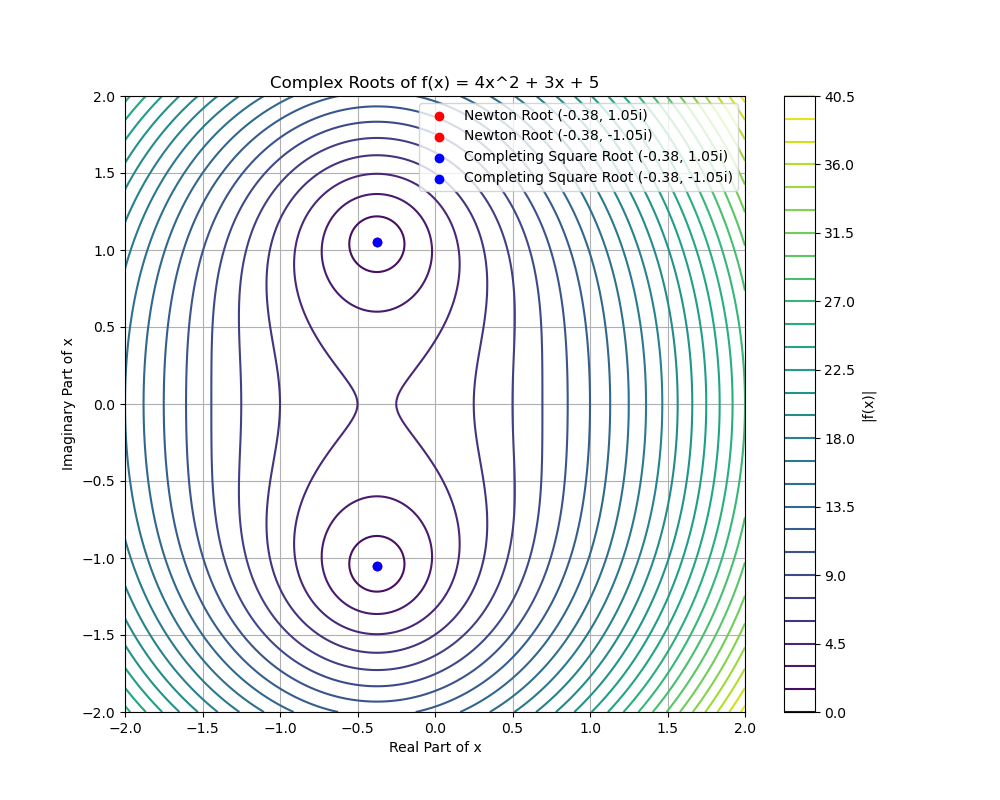
\includegraphics[width=\columnwidth]{figs/Fig2.png}
			\caption{Finding roots using completing squre's and newton's method}
		\label{stemplot}
	\end{figure}
\section*{Solution (Eigenvalue Method - QR Decomposition)}

QR decomposition is a technique in linear algebra to decompose a matrix \( C \) into an orthogonal matrix \( Q \) and an upper triangular matrix \( R \), such that:
\[
C = QR
\]
Here, we use it to iteratively find the eigenvalues of the companion matrix, which correspond to the roots of the quadratic equation.

---

\subsection*{Steps for QR Decomposition}

\text{Step 1: Define the Companion Matrix}

For the quadratic equation:
\[
x^2 + \frac{3}{4}x + \frac{5}{4} = 0
\]
The companion matrix \( C \) is:
\[
C =
\begin{bmatrix}
0 & -\frac{5}{4} \\
1 & -\frac{3}{4}
\end{bmatrix}
\]

---

\text{Step 2: Perform QR Decomposition}

Decompose \( C \) into:
\[
C = QR
\]
where:
- \( Q \) is an orthogonal matrix (\( Q^T Q = I \)),
- \( R \) is an upper triangular matrix.

For a \( 2 \times 2 \) matrix, compute \( Q \) and \( R \) as follows:
1. Normalize the first column of \( C \) to obtain \( q_1 \):
\[
q_1 = \frac{\vec{c_1}}{\|\vec{c_1}\|}
\]
where \( \vec{c_1} \) is the first column of \( C \) and \( \|\vec{c_1}\| \) is its norm.

2. Orthogonalize the second column of \( C \) against \( q_1 \), and normalize to get \( q_2 \):
\[
q_2 = \frac{\vec{c_2} - (\vec{c_2} \cdot q_1)q_1}{\|\vec{c_2} - (\vec{c_2} \cdot q_1)q_1\|}
\]

3. Construct \( Q = [q_1 \, q_2] \).

4. Compute \( R \) using:
\[
R = Q^T C
\]

---

\text{Step 3: Update the Matrix}

Reform the matrix \( C \) by reversing the order of multiplication:
\[
C' = RQ
\]
This step retains the eigenvalues of the original matrix \( C \).

---

\text{Step 4: Iterate the QR Algorithm}

Repeat the process:
1. Decompose \( C' \) into \( Q'R' \).
2. Form \( C'' = R'Q' \).
3. Continue until \( C^{(k)} \) converges to an upper triangular matrix.

---

\text{Step 5: Extract the Eigenvalues}

When the matrix \( C^{(k)} \) becomes upper triangular, the diagonal entries are the eigenvalues of \( C \). For the given quadratic equation, these eigenvalues are:
\[
\boxed{\lambda_1 = \frac{-3 + i\sqrt{71}}{8}, \quad \lambda_2 = \frac{-3 - i\sqrt{71}}{8}}
\]
These eigenvalues correspond to the roots of the quadratic equation \( 4x^2 + 3x + 5 = 0 \).

---

\text{Note: Convergence of the QR Algorithm}

The QR algorithm converges for most matrices, particularly when the matrix is symmetric or normal. For the companion matrix, convergence is achieved after a finite number of steps since it is a small \( 2 \times 2 \) matrix.






\end{document}

